\documentclass[12pt,a4paper,onecolumn]{report}
\usepackage[utf8]{inputenc}
\usepackage{amsmath}
\usepackage{amsfonts}
\usepackage{amssymb}
\usepackage[pdftex]{graphicx}  
\usepackage{float}
\title{Report}
\begin{document}
\author{Shokoofeh Pourmehr}
\chapter*{Advanced Lane Following}
\subsubsection*{Test Images}
Below is a grid of all test images. I have applied all the steps on each test image and included the result in this report.

\begin{figure}[H]
\centering
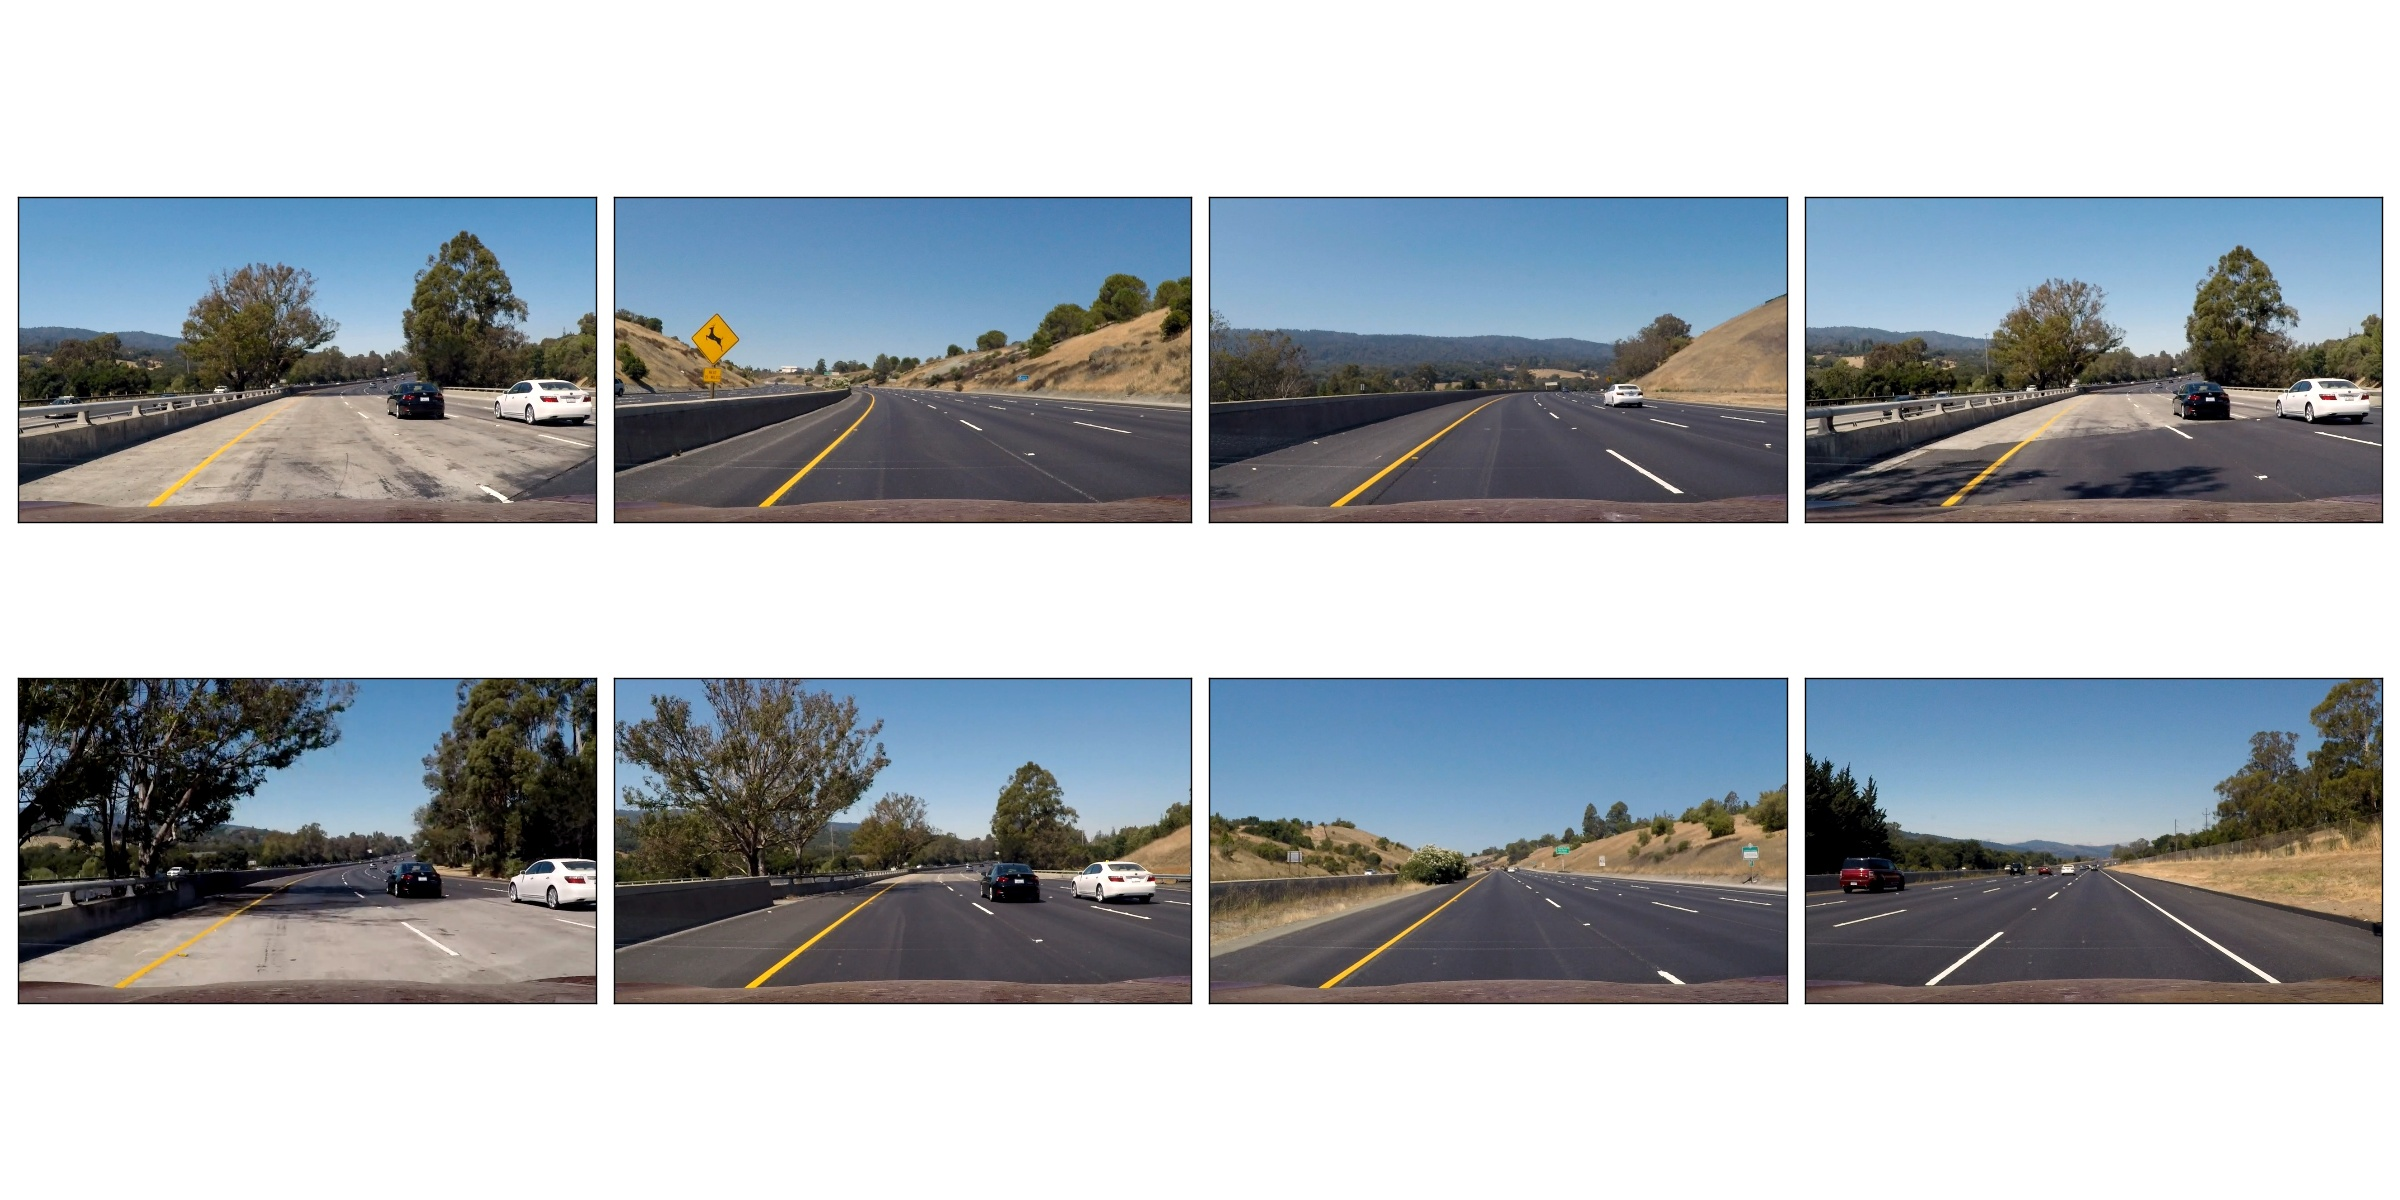
\includegraphics[width=\textwidth]{output_images/grid_images/grid_test_images.jpg}
\caption{Test Images}
\end{figure}

\subsubsection*{Camera Calibration and Distortion Correction}
First I calibrated the camera using calibration images and saved the camera calibration matrix and distortion coefficients so I don't need to compute these again, and to apply them to undistort each new image.

\begin{figure}[H]
\centering
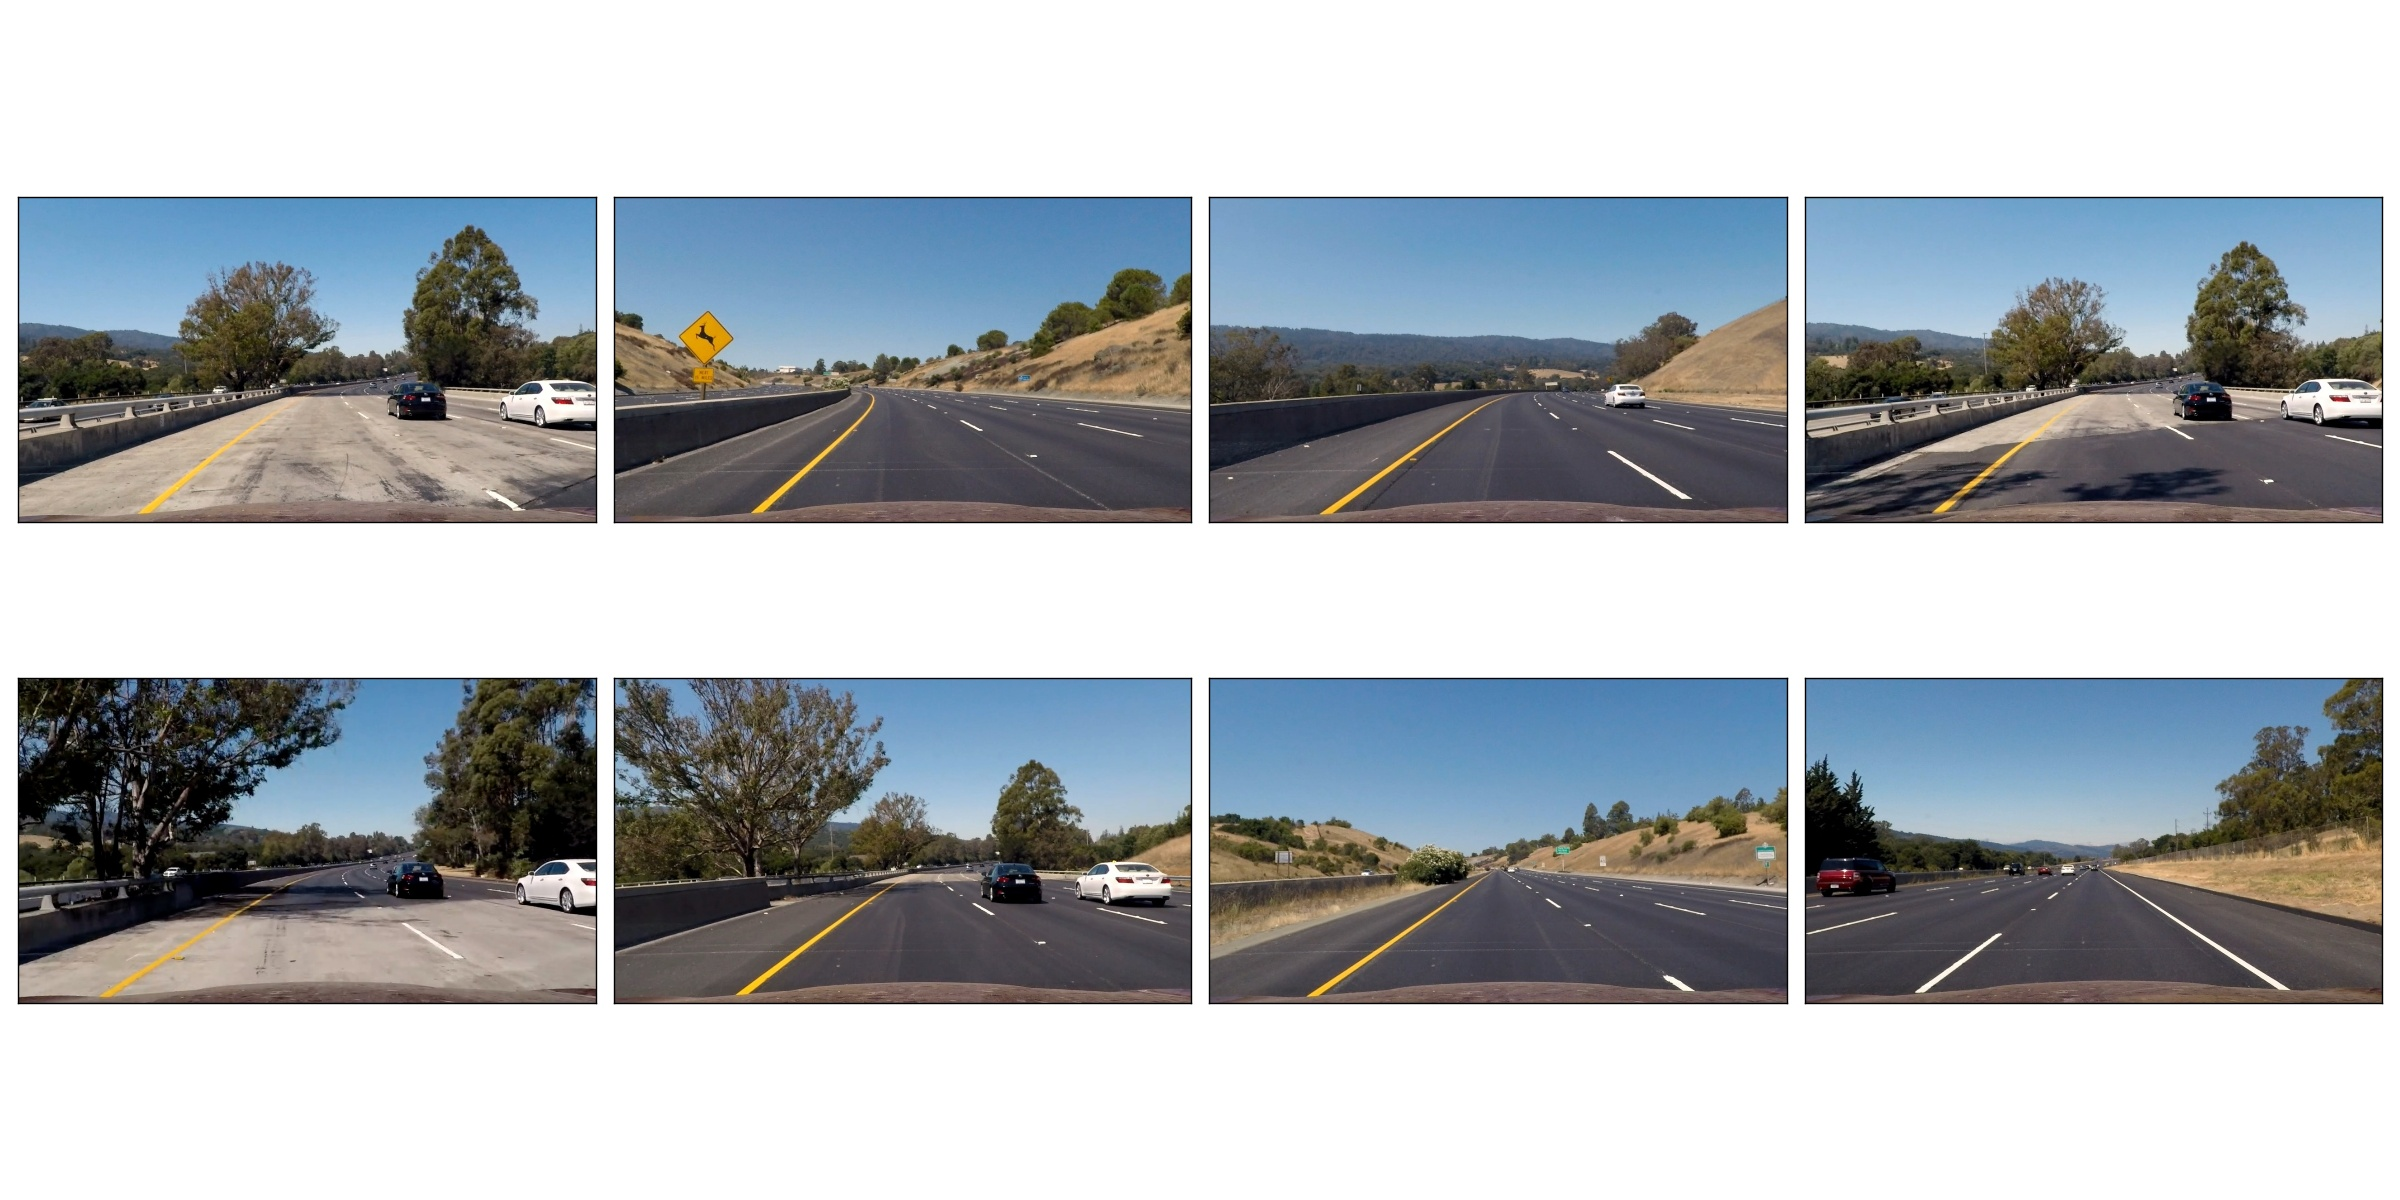
\includegraphics[width=\textwidth]{output_images/grid_images/grid_undistorted_images.jpg}
\caption{Undistorted Images: Applied distortion correction on test images}
\end{figure}


\subsubsection*{Color and gradient threshold}

As the second step I applied color and gradient thresholds to create a binary image. I tried out various combinations of color and gradient thresholds to generate a binary image where the lane lines are clearly visible. The results are visualized in Figure 3.

\begin{figure}[H]
\centering
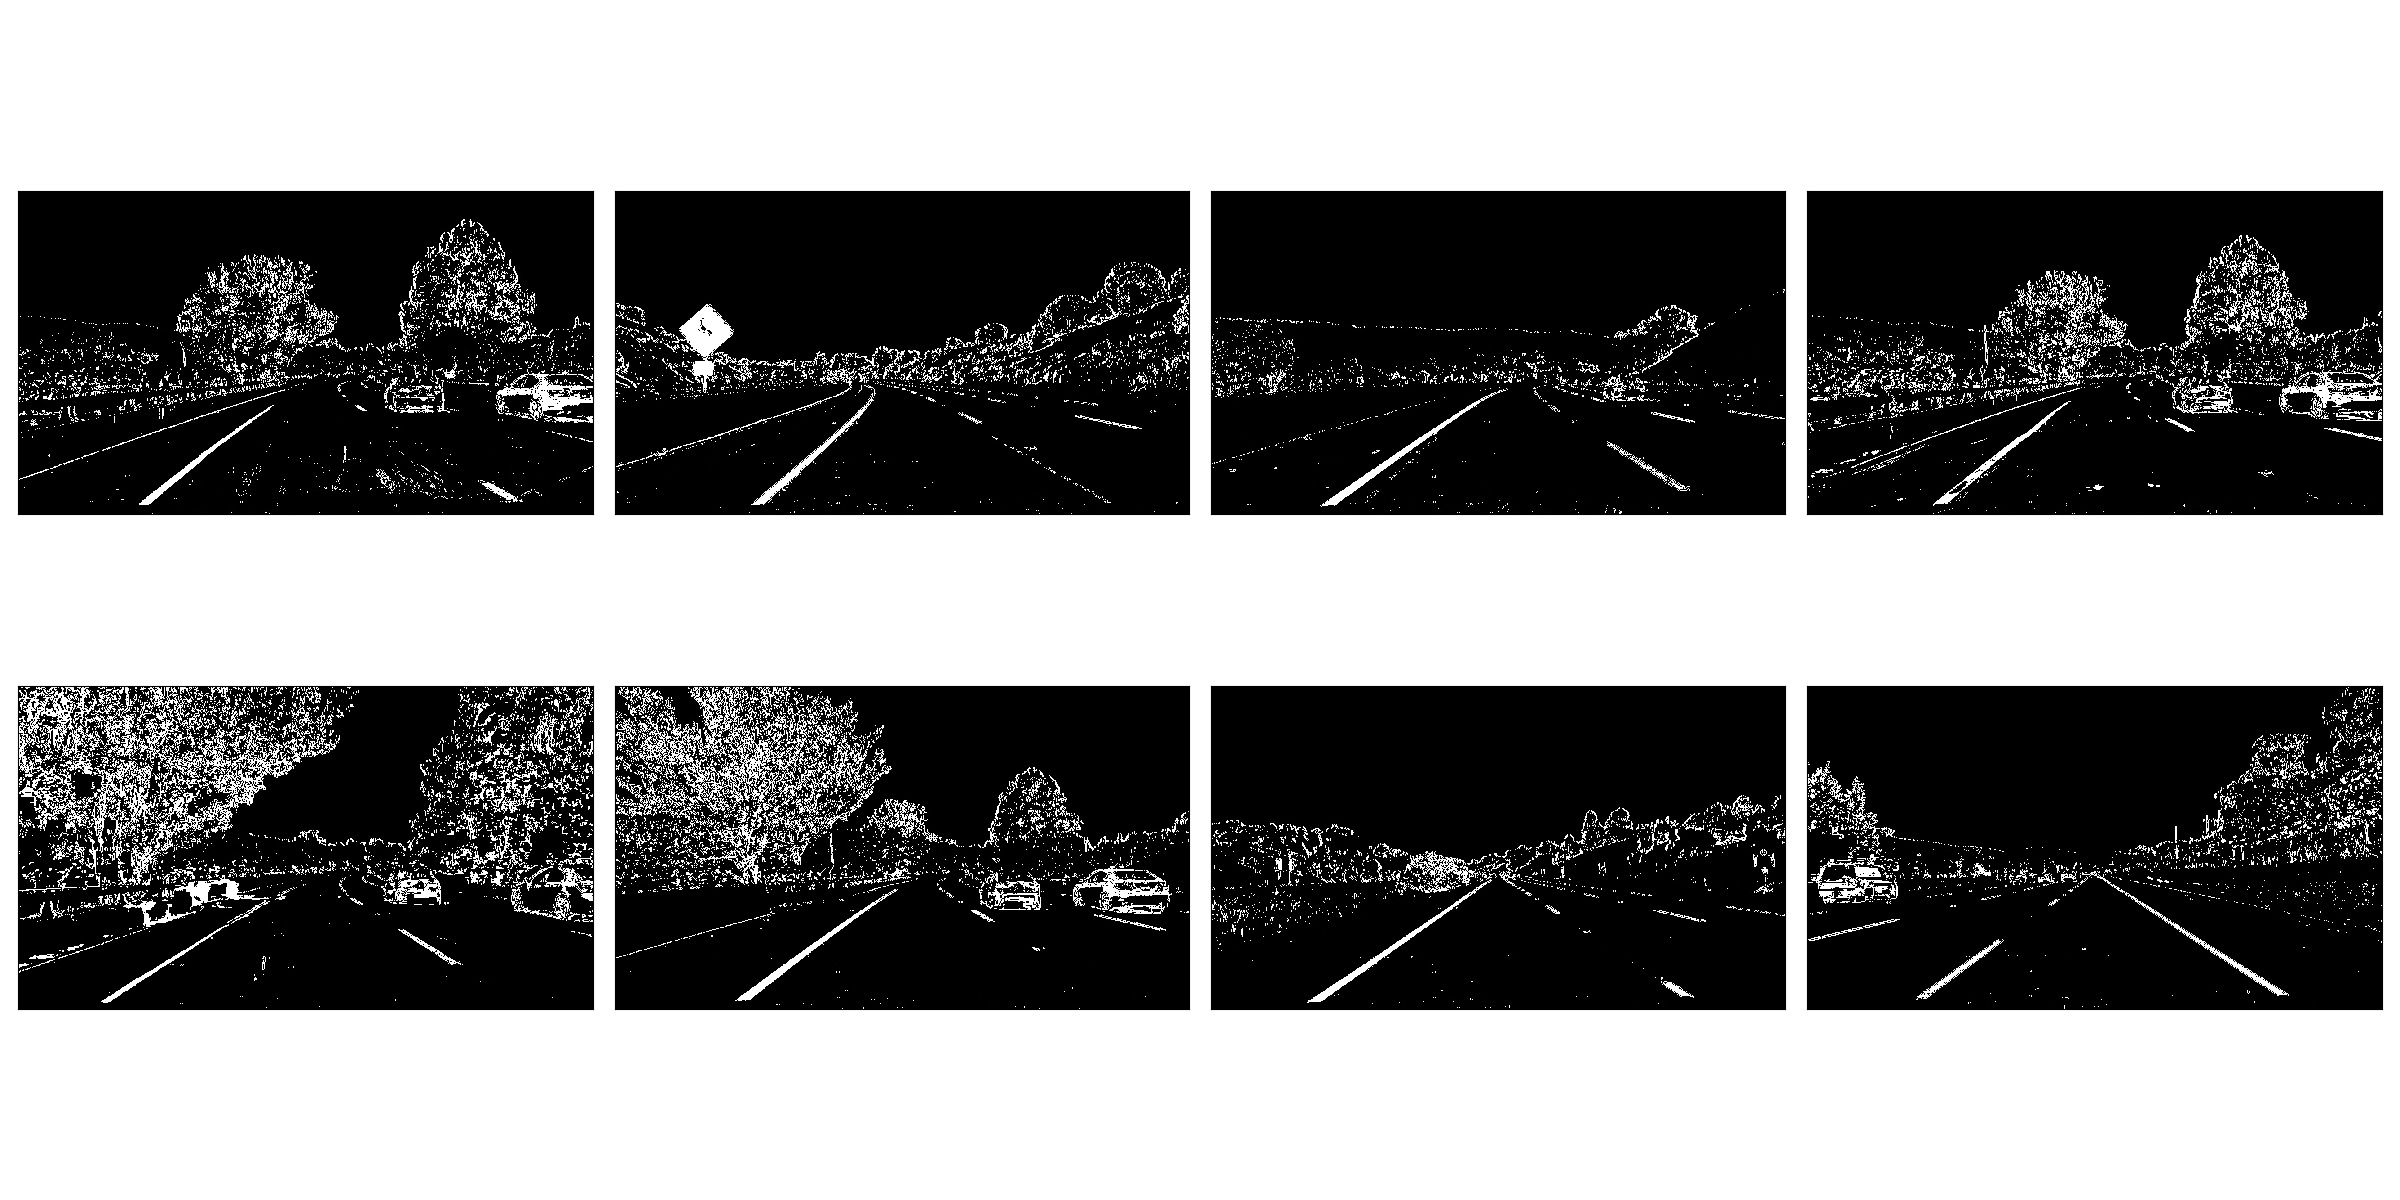
\includegraphics[width=\textwidth]{output_images/grid_images/grid_binary_image.jpg}
\caption{Binary Images: Applied color and gradient thresholds on undistorted images}
\end{figure}


\subsubsection*{Perspective transform}
I applied perspective transform on binary images to get the bird's eye view representation of an image (Figure 4). For each test image I chose the four points separately, using an interactive method, and saved the transformation matrices to be used later. But for the test video I only chose the four points for the first frame and saved the warped and unwarp matrixes to be used for rest of the videp frames.  

\begin{figure}[H]
\centering
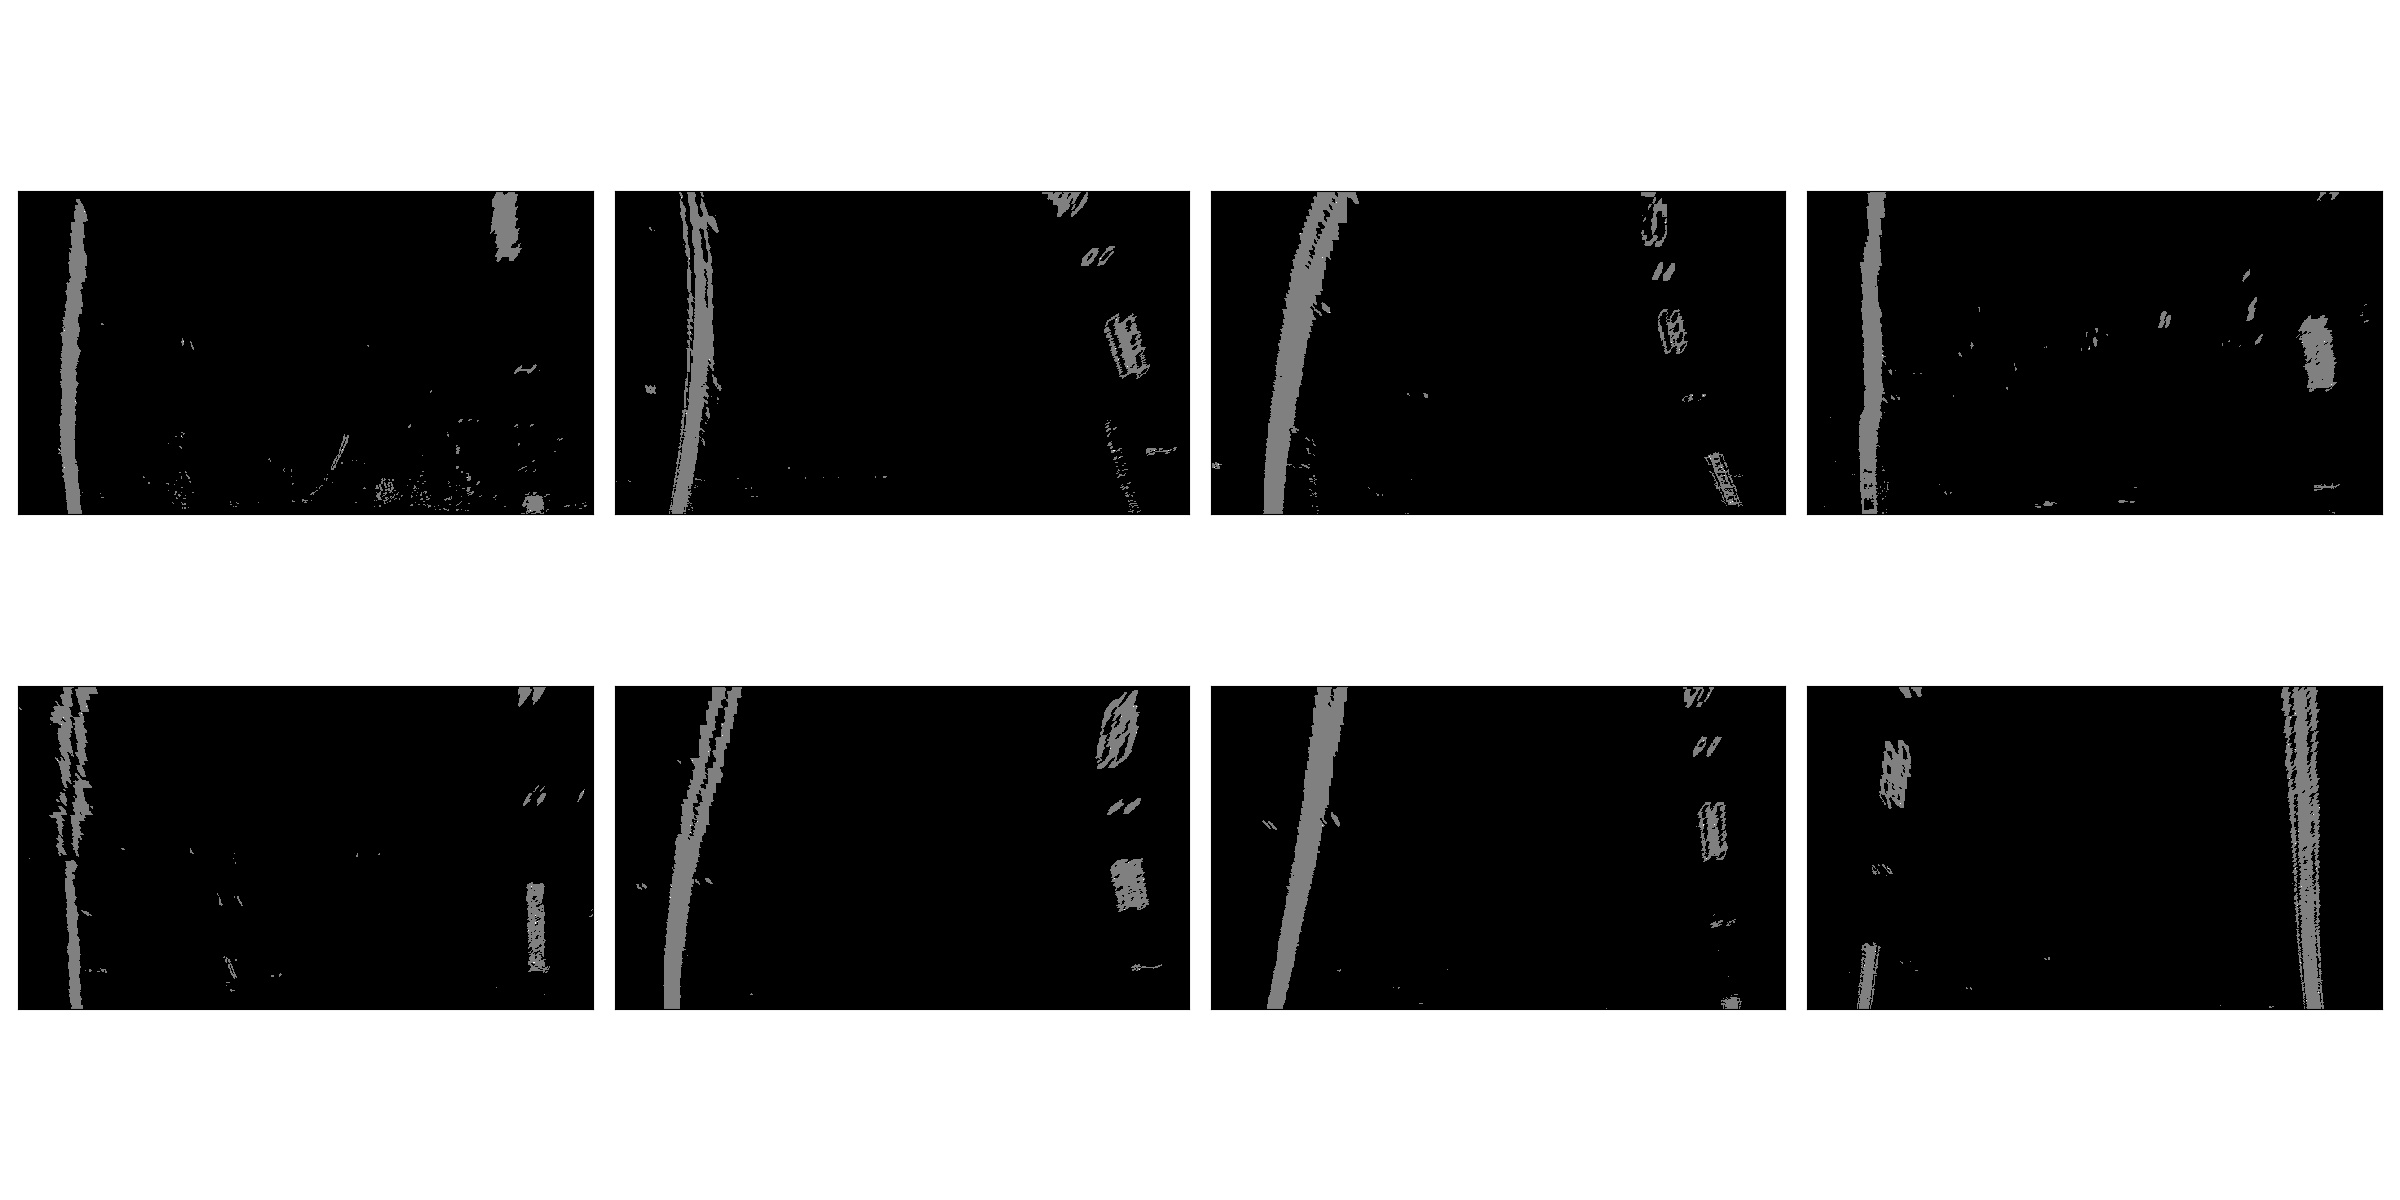
\includegraphics[width=\textwidth]{output_images/grid_images/grid_binary_warped_image.jpg}
\caption{Warped Images: }
\end{figure}

\begin{figure}[H]
\centering
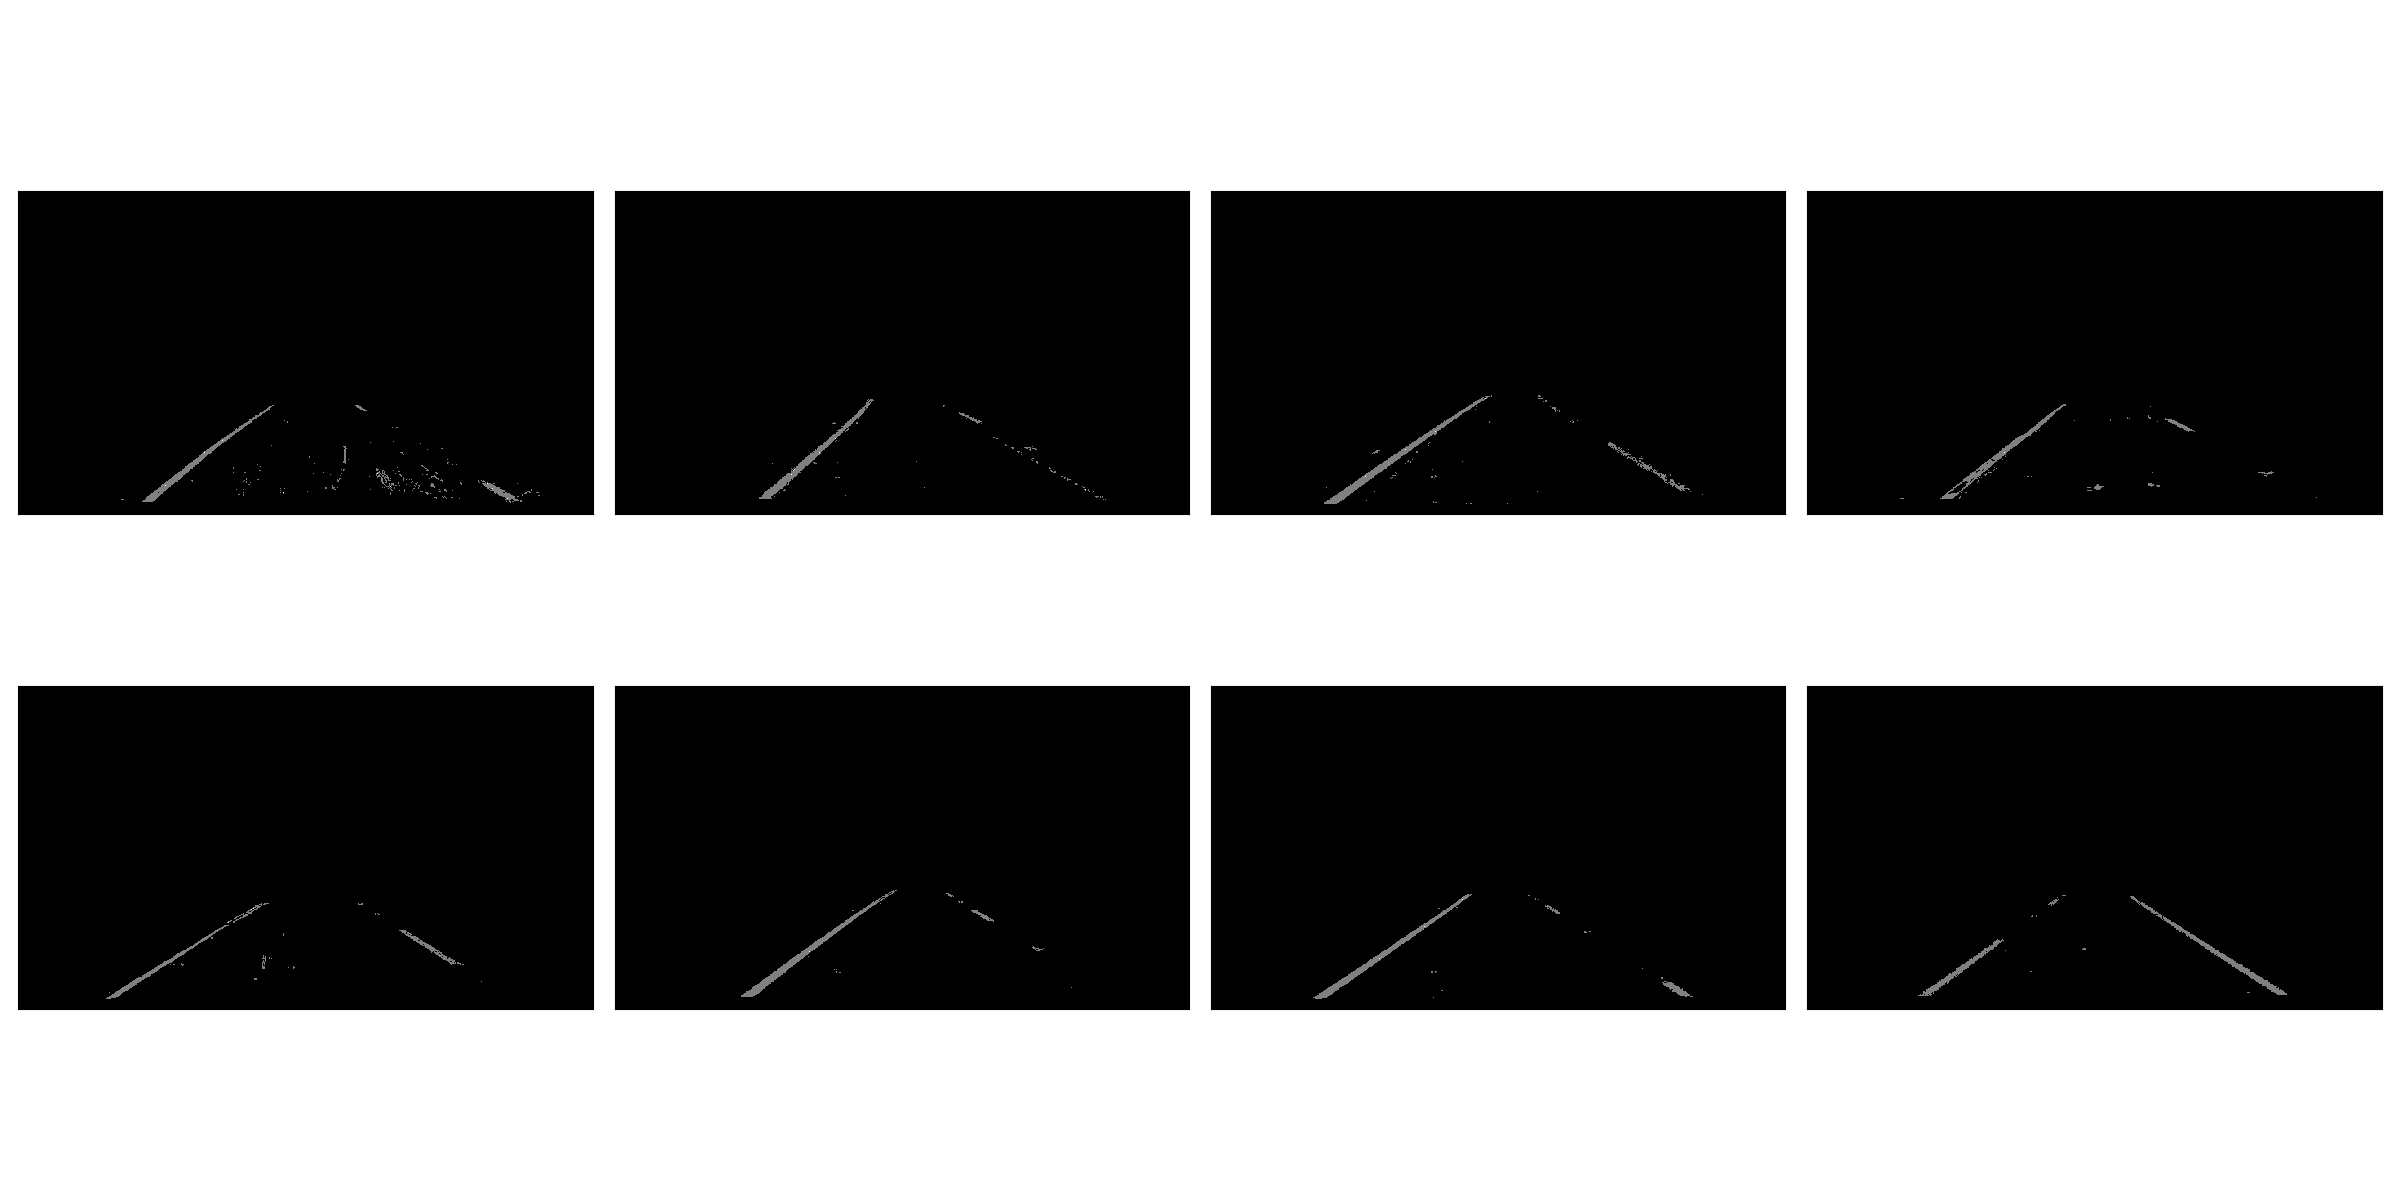
\includegraphics[width=\textwidth]{output_images/grid_images/grid_unwarped_image.jpg}
\caption{Unwarped Images}
\end{figure}


\subsubsection*{Detect lane lines}

After applying calibration, thresholding, and a perspective transform to test images, I used sliding window method to find the pixels that are part of the lines. First I took a histogram along all the columns in the lower half of the image to find the 
\begin{figure}[H]
\centering
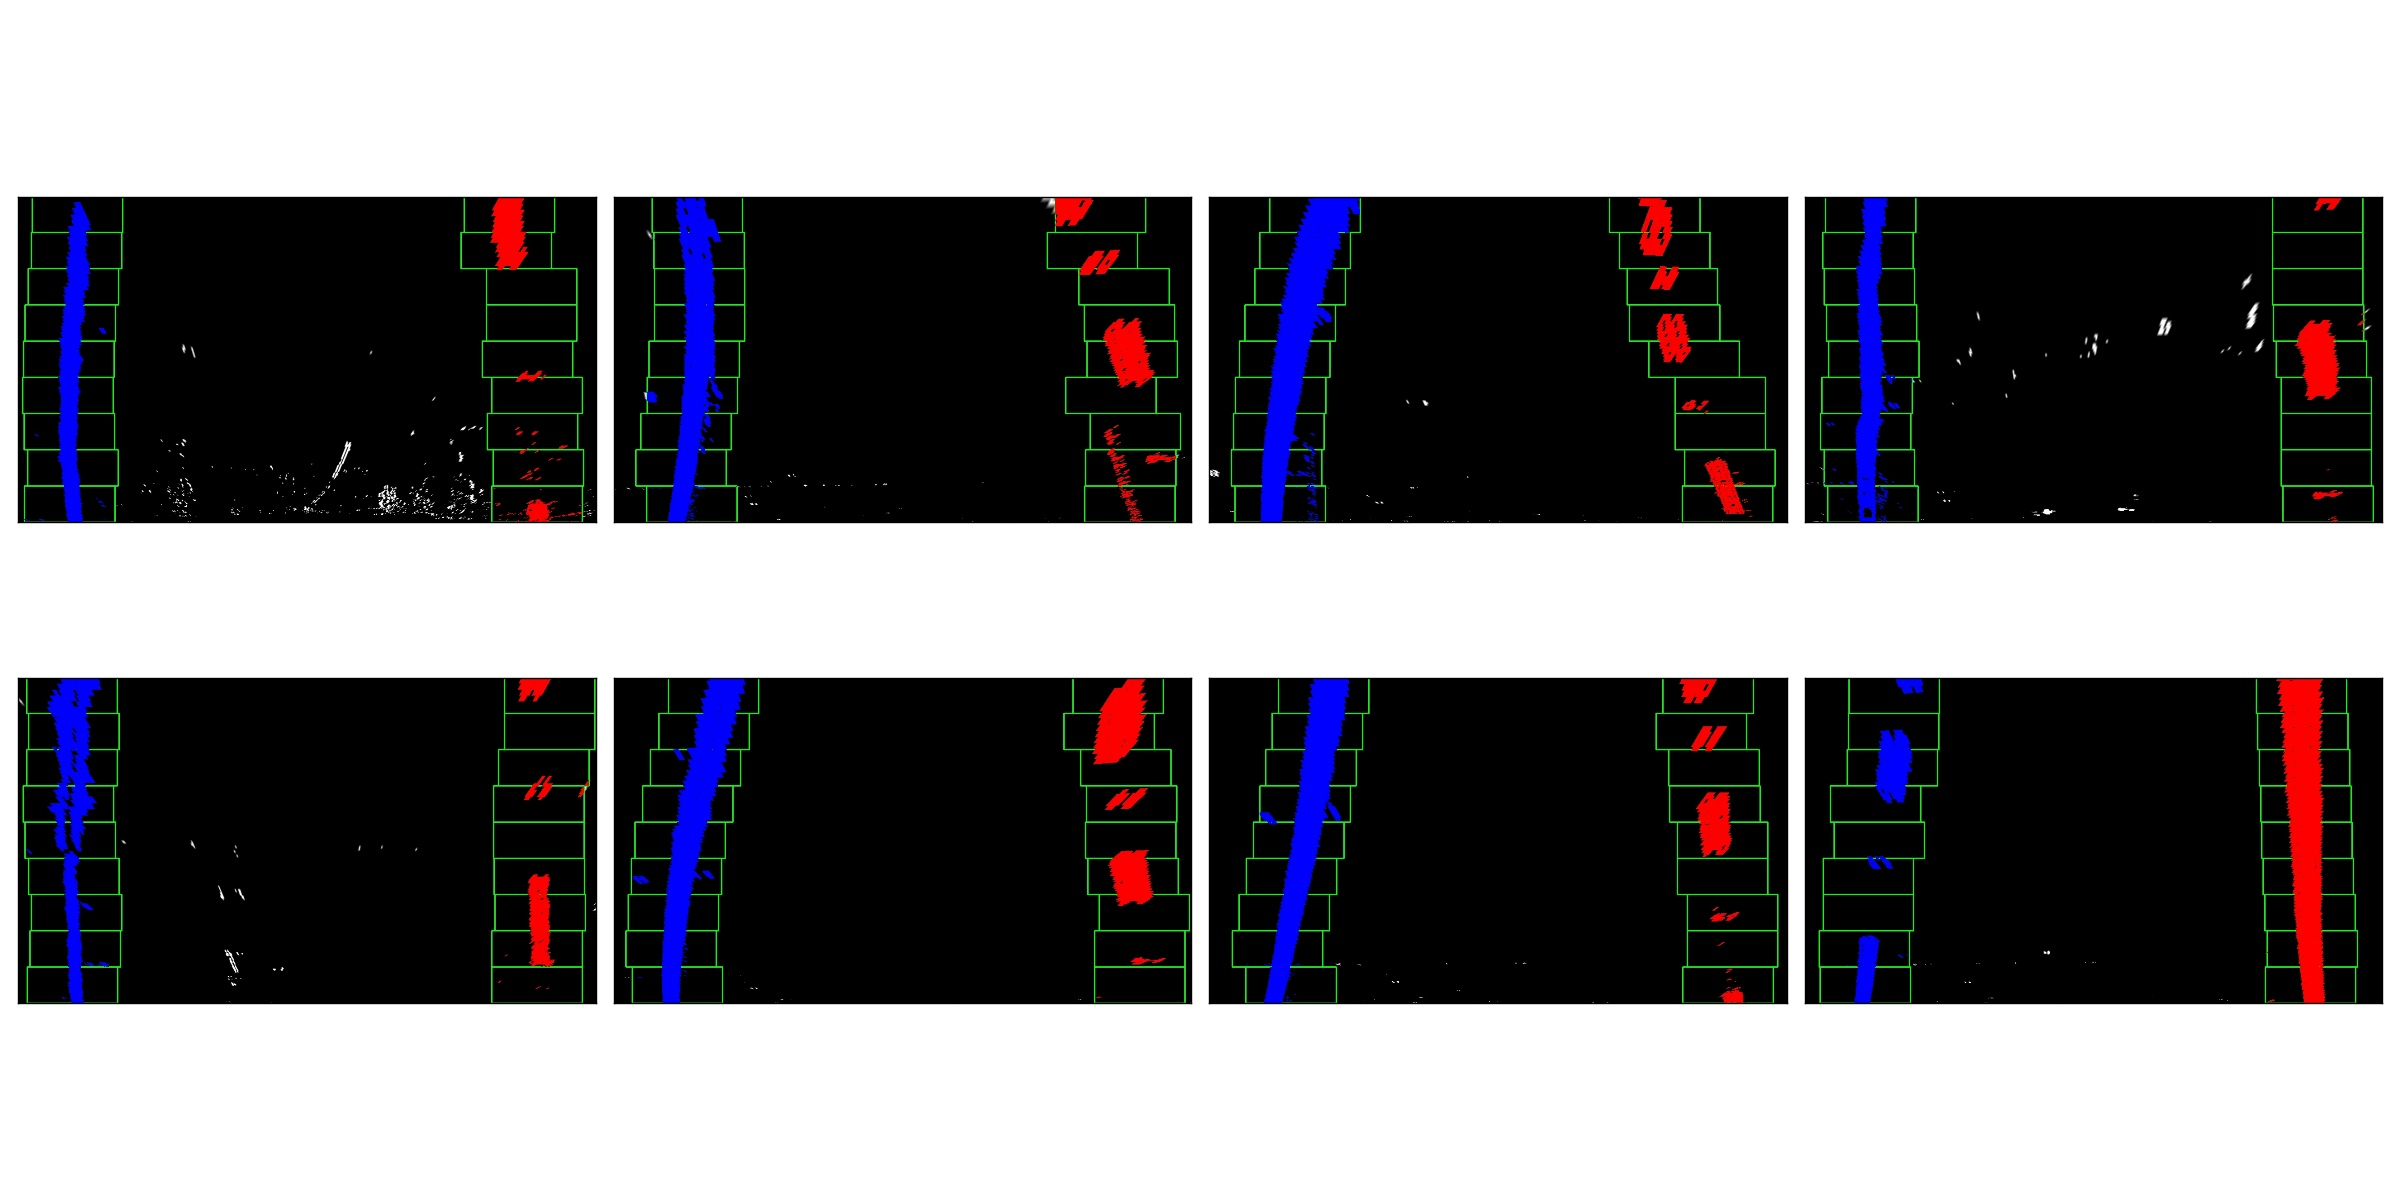
\includegraphics[width=\textwidth]{output_images/grid_images/grid_window_image.jpg}
\caption{Detected lines using sliding window method}
\end{figure}

\begin{figure}[H]
\centering
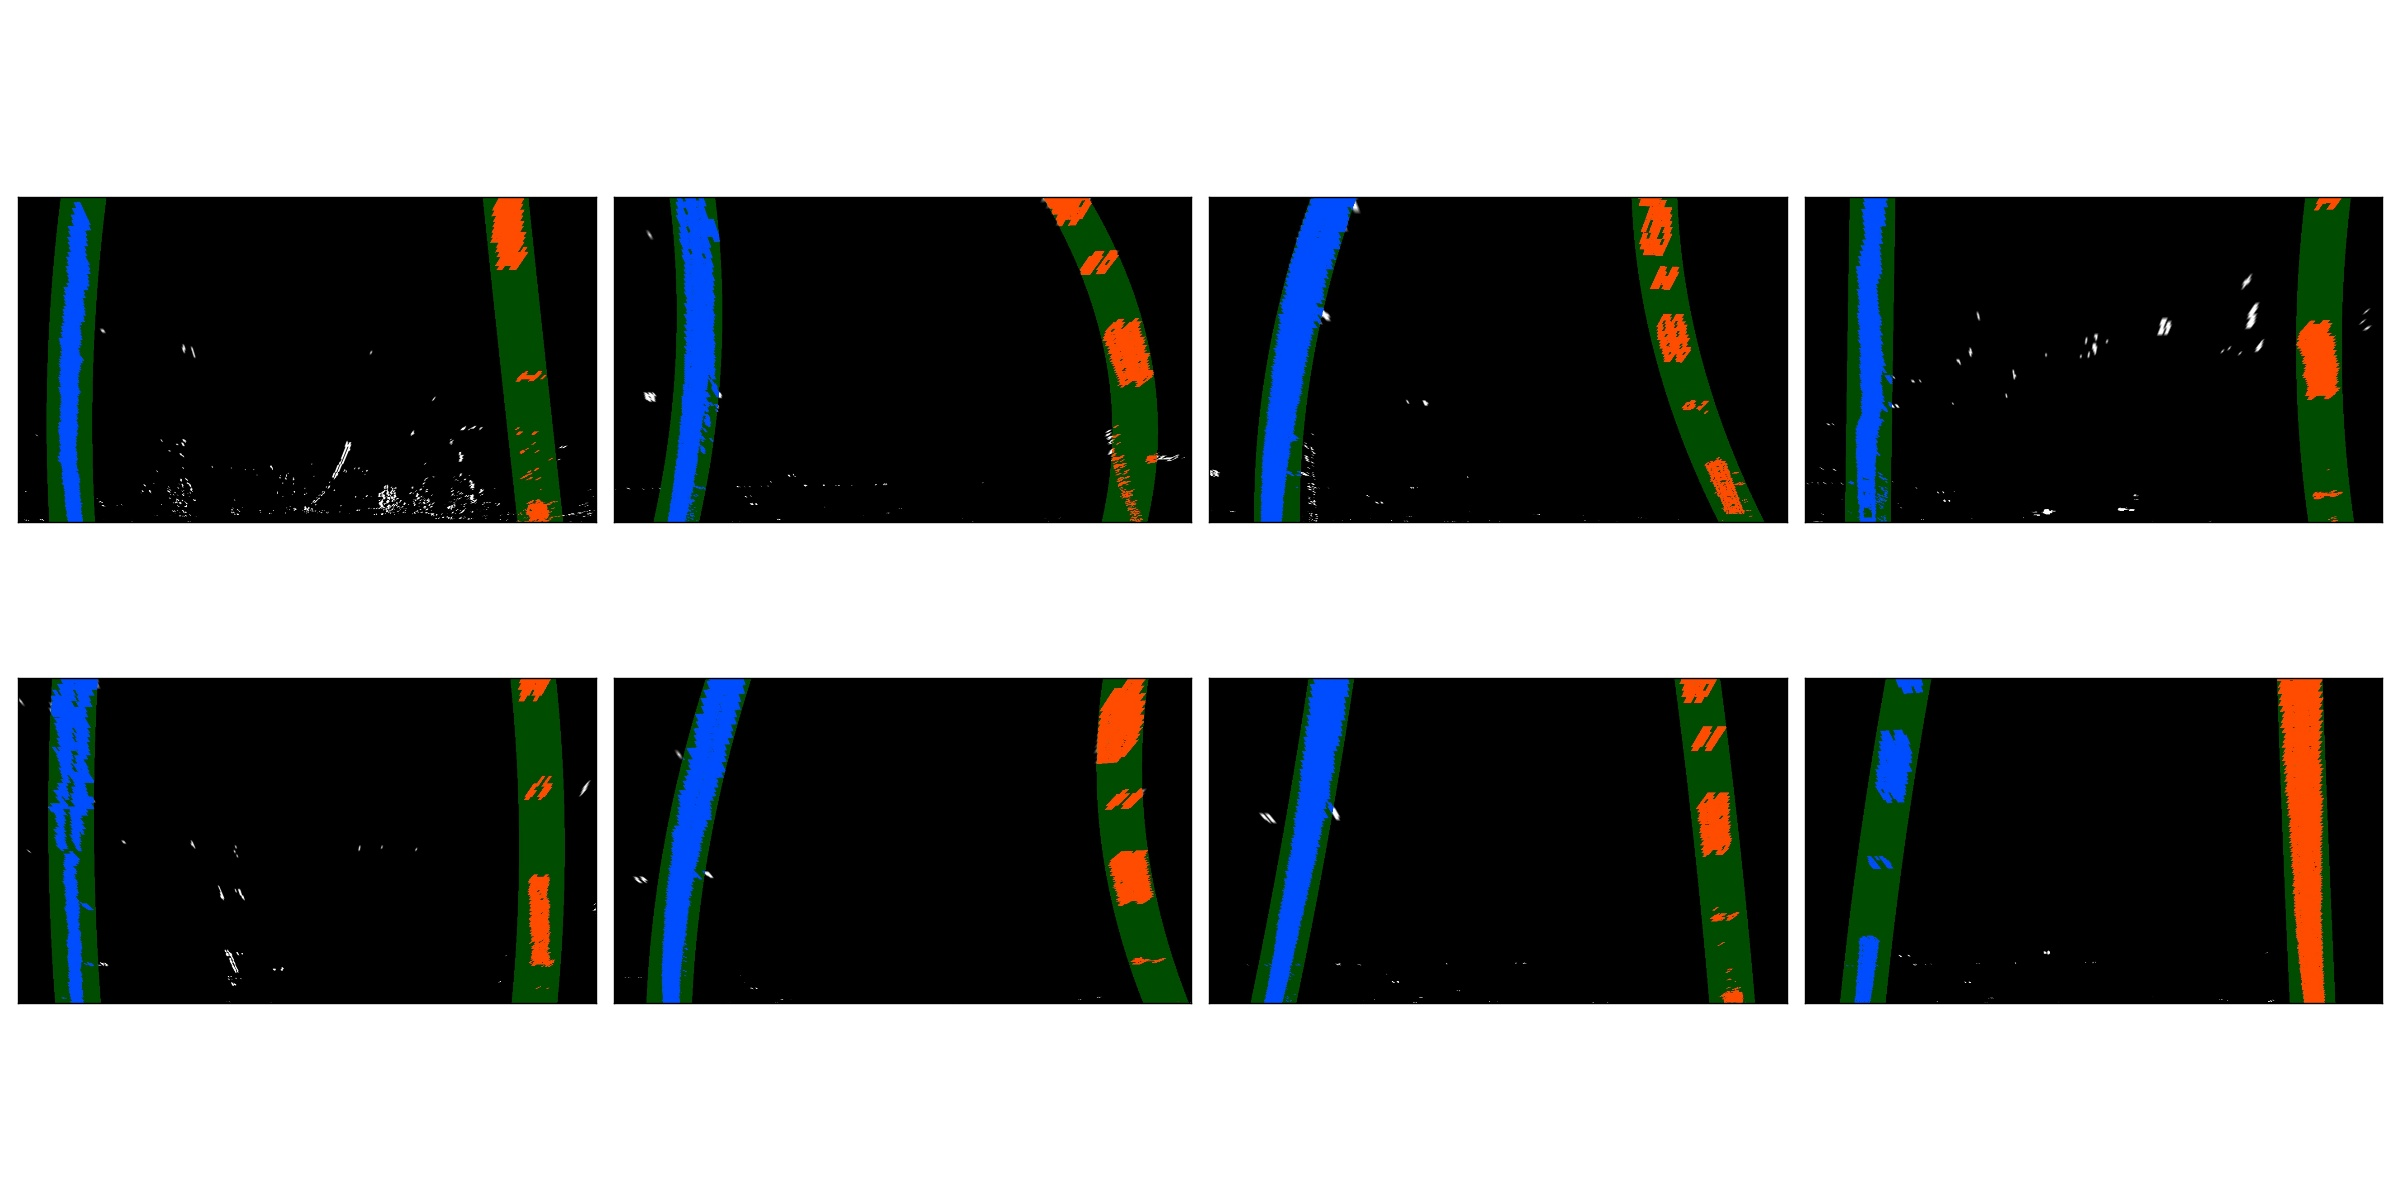
\includegraphics[width=\textwidth]{output_images/grid_images/grid_line_images.jpg}
\caption{Detected lines}
\end{figure}

\subsubsection*{Determine the lane curvature}
\begin{figure}[H]
\centering
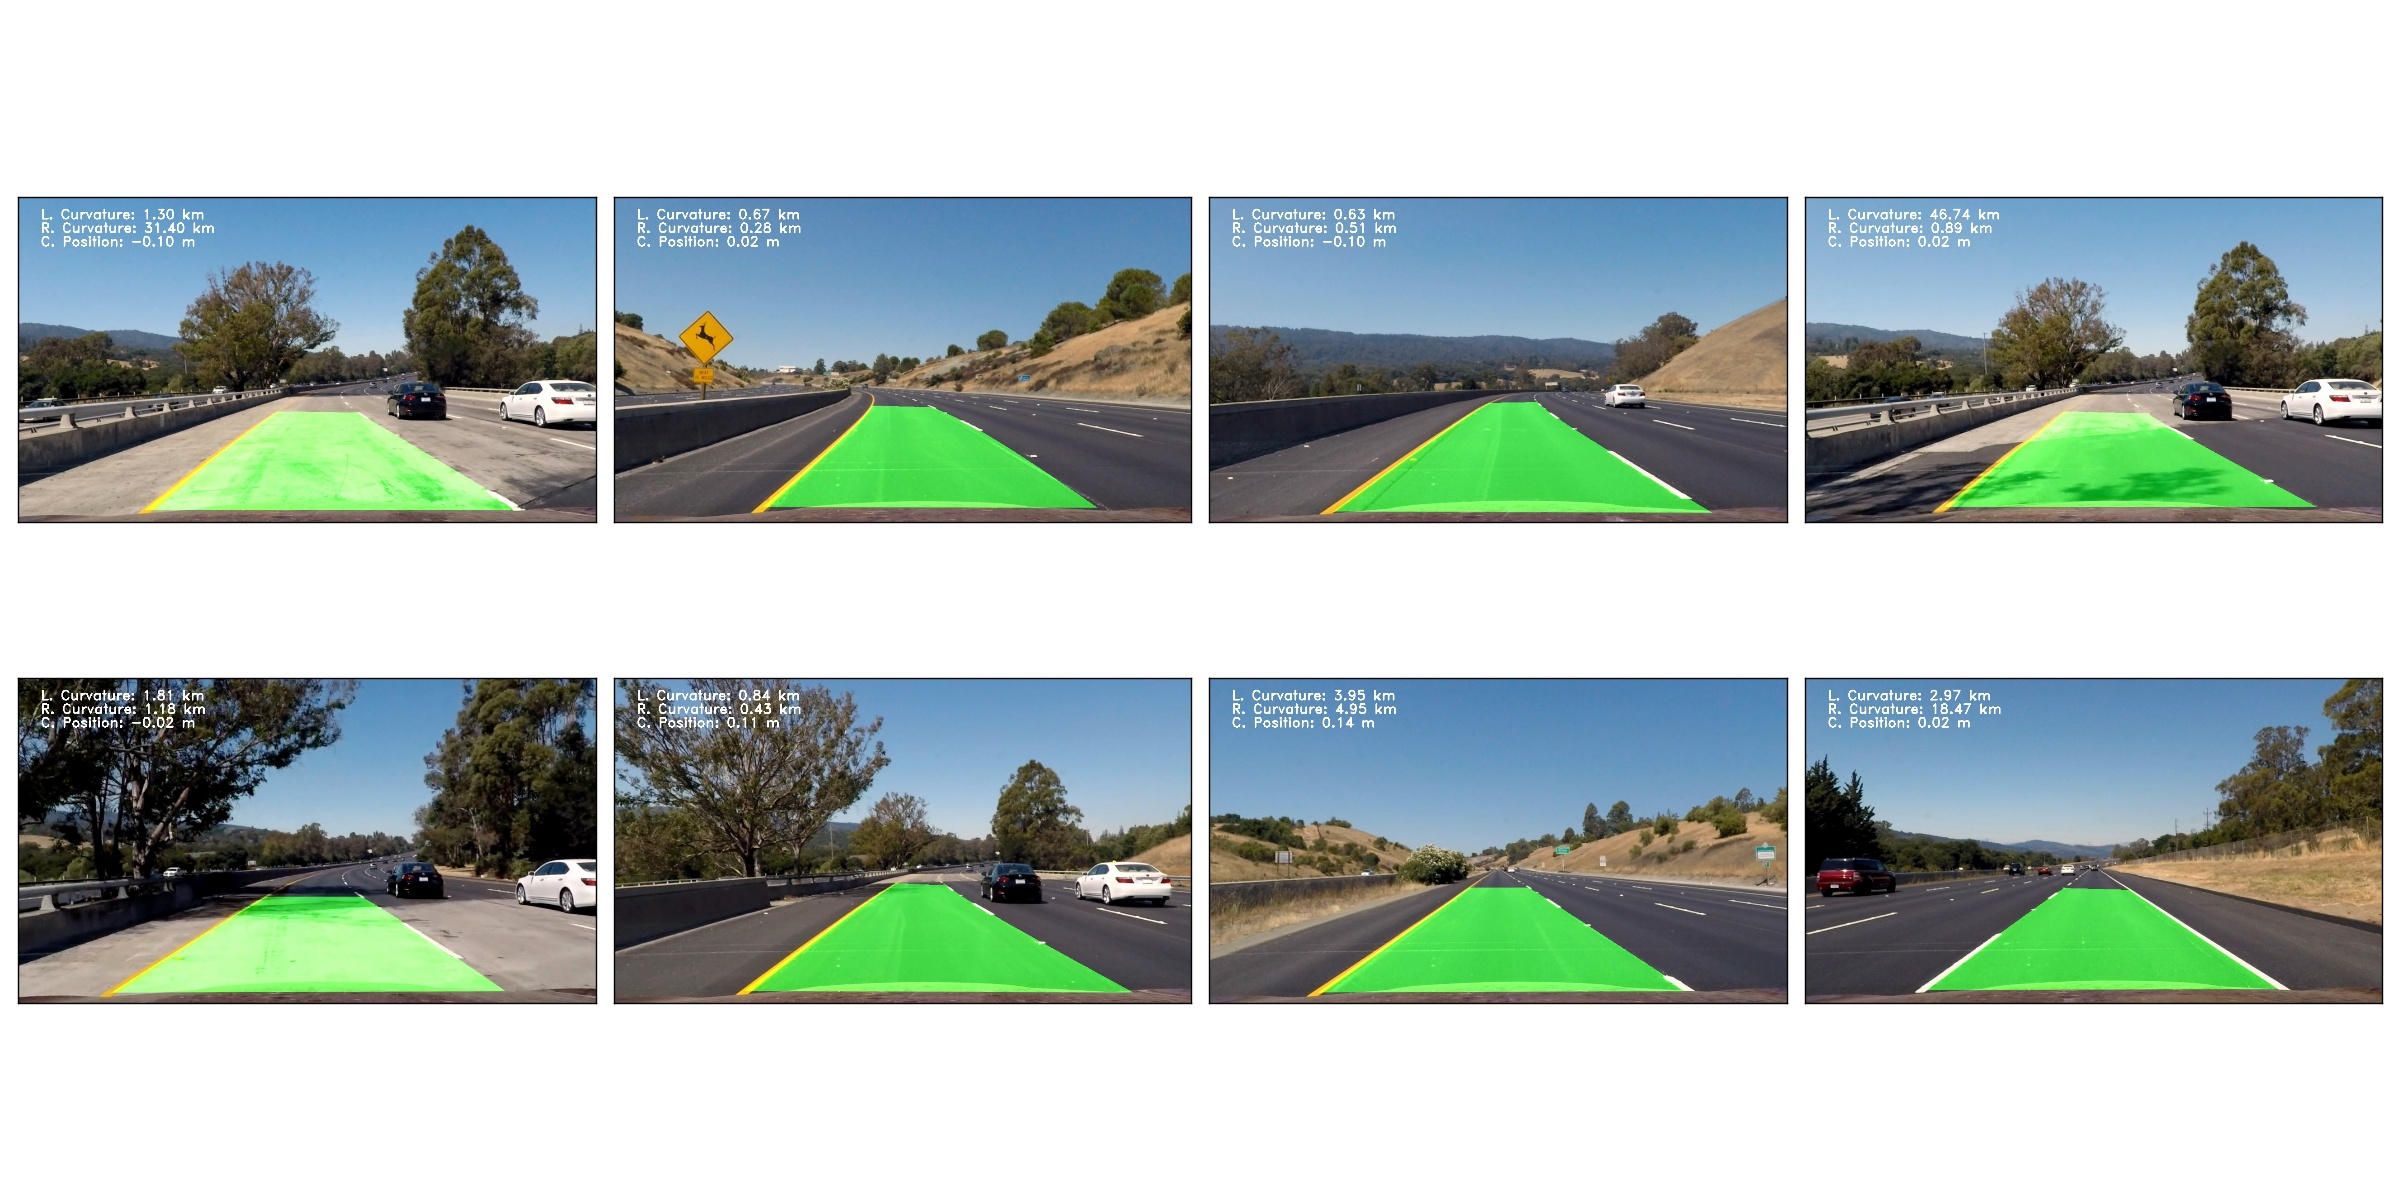
\includegraphics[width=\textwidth]{output_images/grid_images/grid_lane_image.jpg}
\caption{Detected lanes}
\end{figure}


\end{document}\grid
